\usetikzlibrary{shapes.geometric}
\usetikzlibrary{positioning}

\newcommand{\apparatus}[4]{\node[square node] (#1) at (#2,#3){#4};
                           \node[port] (#1+) at (#2 + 0.375, #3 + 0.5){+};
                           \node[port] (#1-) at (#2 + 0.375, #3 - 0.5){-};}

\part{Background}
\chapter{Stern-Gerlach Experiments}
\section{Stern-Gerlach Backgorund}
TODO
\section{Stern-Gerlach Measurement}

We begin by comparing standard and consistent descriptions of measuring a quantum states' spin along one axis using a Stern-Gerlach apparatus. In standard quantum mechanics, the act of measurement plays a special role in assigning probabilities to the outcome and the evolution of the state through the probability and projection postulates.

The probability postulate assigns probabilities to each measurement by taking the inner product of the state $\ket{n}$ corresponding to a measruement result $n$ and $\ket{\psi}$:
\begin{align}
    \mathcal{P}_n = |\braket{n|\psi}|^2
\end{align}

The projection postulate describes an instantaneous evolution of the input state to an output state that corresponds to an allowed measruement value. If input $\ket{\psi}$ is measured to have spin $n$ (up or down), then the new state is
\begin{align}
    \ket{\psi}^\prime = \frac{P_n\ket{\psi}}{\sqrt{\bra{\psi}P_n\ket{\psi}
    }}
\end{align}
where $P_n = \ket{n}\bra{n}$ is the projection operator for state $\ket{n}$. This operation projects $\ket{\psi}$ onto $\ket{n}$, then divides by the magnitude of that projection. The end result is that $\ket{\psi}$ becomes the normalized state $\ket{n}$ corresponding to measuring spin $n$, which is shown by the states exiting the each apparatus.

\begin{figure}
\centering\CaptionFontSize
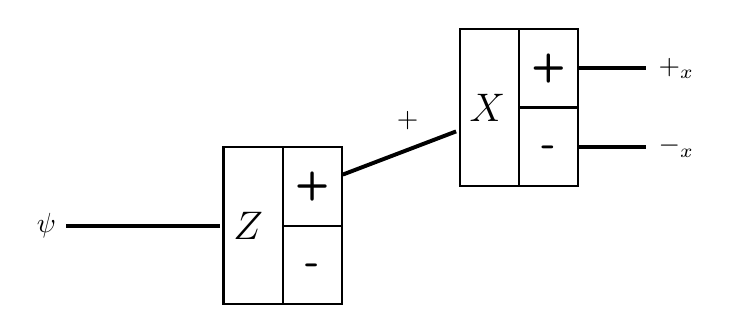
\begin{tikzpicture}[shorten >=1pt,auto, thick,
     square node/.style={rectangle, minimum height=2cm, minimum width=1.50cm, text width = 1.25cm, draw, font=\sffamily\Large\bfseries},
     port/.style={rectangle, draw,  minimum height=1cm, minimum width=0.75cm, font=\sffamily\Large\bfseries},
     wf/.style={rectangle, minimum height=1cm}]
    \apparatus{1}{3}{0}{$Z$};
    \apparatus{2}{6}{1.5}{$X$};

    \node[wf] (w0) at (0,0) {$\ket{\psi}$};
    \node[wf] (w1) at (8, 2.0) {$\ket{+}_x$};
    \node[wf] (w2) at (8, 1.0) {$\ket{-}_x$};

    \draw[line width=0.5mm] (w0) -- (1);

    \draw[line width=0.5mm] (1+) -- (2) node [near end] {$\ket{+}$};

    \draw[line width=0.5mm] (2+) -- (w1);
    \draw[line width=0.5mm] (2-) -- (w2);
\end{tikzpicture}
\caption[Insert an abbreviated caption here to show in the List of Figures]
{Demonstrating renormalizing upon measurment in standard quantum mechanics}
\label{Figure:Intro:FigureExampleA}
\end{figure}

TODO: show probability computations
TODO: explain how measurement is not itself modeled as a physical process, and we are directed to use these postulates upon poorly defined "measurement"

In consistent quantum theory, measurement is modeled as a physical process. Each Stern-Gerlach apparatus has its own detector Hilbert space, containing orthonormal states representing each measurement result. Let the state space of the $z$ apparatus be represented by ${\mathcal{H}_D}_z =  \{\ket{D_z}_+, \ket{D_z}_-\}$ where $_+\braket{D_z|D_z}_+=1$ and $_+\braket{D_z|D_z}_-=0$. ${\mathcal{H}_D}_x$ is similarly defined. Each detector state is orthogonal to states in seperate detector spaces.

The act of measurement is described by correlating the detector states with the corresponding quantum states. The system then evolves by
\begin{align}
    \nonumber V: \\
    & \nonumber \mathcal{H}_s \mapsto \mathcal{H}_s \otimes \mathcal{H}_D \\
    & \ket{\psi} = \sum_{n} P_n\ket{\psi} \mapsto \sum_{n} P_n\ket{\psi} \otimes \ket{D}_n
\end{align}

Measurment is now described by an abstract physical process. In this model, it is now feasible for "state collapse" to occur independent of physicists conducting clever experiments.

To compute probabilities of each outcome, we sum the magnitudes of each branch wavefunction that includes the corresponding detector state. This is accomplished by finding the trace of the projection operator of that detector state acting on the projection operator or the overall evolved state.
\begin{align}
    \mathcal{P}_n = Tr(P^D_n \cdot V\ket{\psi}\bra{\psi}V^\dagger)
\end{align}

In this simple Stern-Gerlach example, there is only one branch wavefunction correlated with each detector state. So, computing probabilities is done by finding the magnitude of each branch wavefunction.

TODO: compute probabilities, show it is equal to std QM

\begin{figure}
\centering\CaptionFontSize
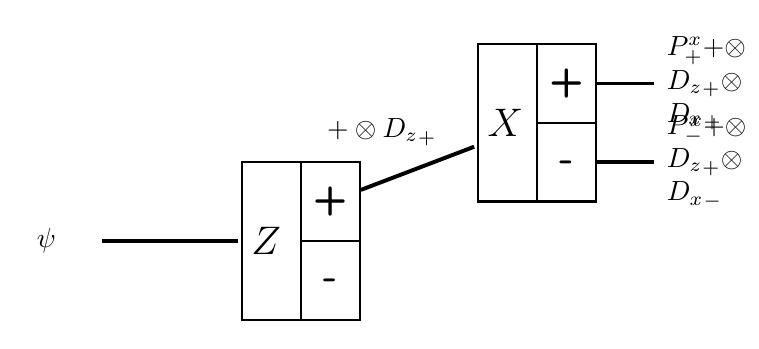
\begin{tikzpicture}[shorten >=1pt,auto, thick,
     square node/.style={rectangle, minimum height=2cm, minimum width=1.50cm, text width = 1.25cm, draw, font=\sffamily\Large\bfseries},
     port/.style={rectangle, draw,  minimum height=1cm, minimum width=0.75cm, font=\sffamily\Large\bfseries},
     wf/.style={rectangle, minimum height=1cm, text width = 0.7cm}]
    \apparatus{1}{3}{0}{$Z$};
    \apparatus{2}{6}{1.5}{$X$};

    \node[wf] (w0) at (0,0) {$\ket{\psi}$};
    \node[wf] (w1) at (8, 2.0) {$P^x_+ \ket{+} \otimes \ket{D_z}_+  \otimes \ket{D_x}_+$};
    \node[wf] (w2) at (8, 1.0) {$P^x_- \ket{+} \otimes \ket{D_z}_+ \otimes \ket{D_x}_-$};

    \draw[line width=0.5mm] (w0) -- (1);

    \draw[line width=0.5mm] (1+) -- (2) node [near end] {$\ket{+} \otimes \ket{D_z}_+$};

    \draw[line width=0.5mm] (2+) -- (w1);
    \draw[line width=0.5mm] (2-) -- (w2);
\end{tikzpicture}
\caption[Insert an abbreviated caption here to show in the List of Figures]
{Demonstrating description of measurment as an abstract physical process in consistent quantum mechanics}
\label{Figure:Intro:FigureExampleB}
\end{figure}

\section{Complementarity}

We now compare standard and consistent quantum mechanics' treatment of the principle of complementarity. Arguably the most fundamental feature of quantum mechanics, the principle of complementarity states that a quantum system has pairs of physical observables which cannot be measured simultaneously. Components of spin on orthogonal axes are complemntary properties, so we examine measurements of succesive Stern-Gerlach experiments.

First, we compute the probabilities of each outcome using standard quantum mechanics. The first apparatus serves as a state preparation device with output $\ket{+}$. By the direction of the projection postulate, the state is renormalized upon each measruement. After measuring a property complementary to what is known (such as spin along $x$, knowing spin along $z$), any information known about the input state is lost; the input state instantaneously changes to the state corresponding to the observed quantity. Consequently, there is an equal probability of observing the final state as $\ket{+}$ or $\ket{-}$ at either final apparatus, even though the state was initially prepared as $\ket{+}$, since
\begin{align*}
    \mathcal{P}_n &= |\braket{+|+}_x|^2 \\
                  &= |\braket{-|+}_x|^2 \\
                  &= |\braket{+|-}_x|^2 \\
                  &= |\braket{-|-}_x|^2 \\
                  &= \frac{1}{4}
\end{align*}
This contradiction with classical intuition is a direct result of the projection postulate. TODO: describe measurement problem.

TODO: Demonstrate complementarity and single framework rule

\begin{figure}
\centering\CaptionFontSize
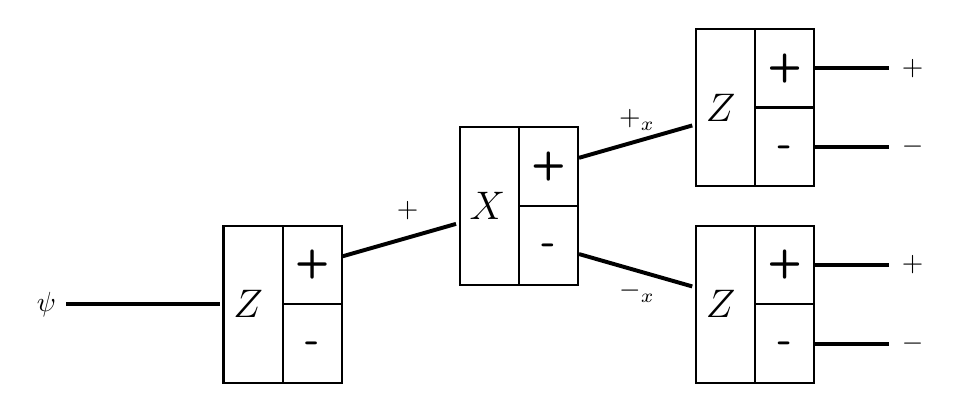
\begin{tikzpicture}[shorten >=1pt,auto, thick,
     square node/.style={rectangle, minimum height=2cm, minimum width=1.50cm, text width = 1.25cm, draw, font=\sffamily\Large\bfseries},
     port/.style={rectangle, draw,  minimum height=1cm, minimum width=0.75cm, font=\sffamily\Large\bfseries},
     wf/.style={rectangle, minimum height=1cm}]
    \apparatus{1}{3}{0}{$Z$};
    \apparatus{2}{6}{1.25}{$X$};
    \apparatus{3}{9}{2.50}{$Z$};
    \apparatus{4}{9}{0}{$Z$};

    \node[wf] (w0) at (0,0) {$\ket{\psi}$};
    \node[wf] (w1) at (11, 3.0) {$\ket{+}$};
    \node[wf] (w2) at (11, 2.0) {$\ket{-}$};
    \node[wf] (w3) at (11, 0.5) {$\ket{+}$};
    \node[wf] (w4) at (11, -0.5) {$\ket{-}$};

    \draw[line width=0.5mm] (w0) -- (1);

    \draw[line width=0.5mm] (1+) -- (2) node [near end] {$\ket{+}$};

    \draw[line width=0.5mm] (2-) -- (4) node [midway, below] {$\ket{-}_x$};
    \draw[line width=0.5mm] (2+) -- (3) node [midway, above] {$\ket{+}_x$};

    \draw[line width=0.5mm] (3-) -- (w2);
    \draw[line width=0.5mm] (3+) -- (w1);
    \draw[line width=0.5mm] (4-) -- (w4);
    \draw[line width=0.5mm] (4+) -- (w3);
\end{tikzpicture}
\caption[Insert an abbreviated caption here to show in the List of Figures]
{Demonstrating complementary measurments in standard quantum mechanics}
\label{Figure:Intro:FigureExampleC}
\end{figure}

\begin{figure}
\centering\CaptionFontSize
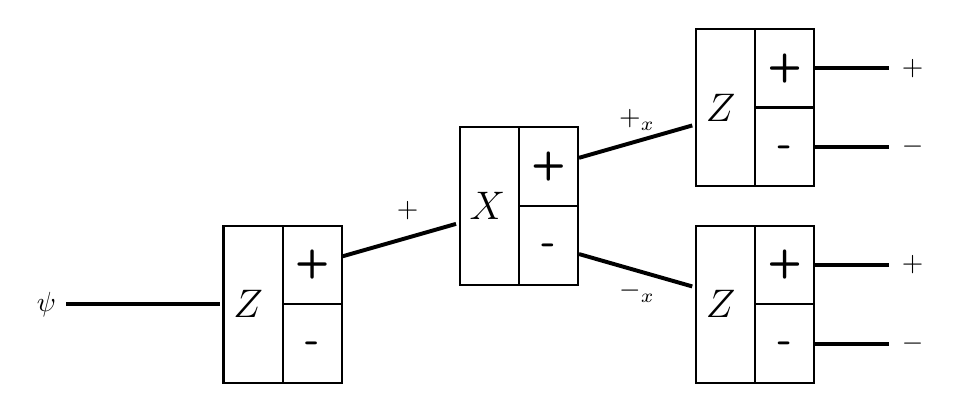
\begin{tikzpicture}[shorten >=1pt,auto, thick,
     square node/.style={rectangle, minimum height=2cm, minimum width=1.50cm, text width = 1.25cm, draw, font=\sffamily\Large\bfseries},
     port/.style={rectangle, draw,  minimum height=1cm, minimum width=0.75cm, font=\sffamily\Large\bfseries},
     wf/.style={rectangle, minimum height=1cm}]
    \apparatus{1}{3}{0}{$Z$};
    \apparatus{2}{6}{1.25}{$X$};
    \apparatus{3}{9}{2.50}{$Z$};
    \apparatus{4}{9}{0}{$Z$};

    \node[wf] (w0) at (0,0) {$\ket{\psi}$};
    \node[wf] (w1) at (11, 3.0) {$\ket{+}$};
    \node[wf] (w2) at (11, 2.0) {$\ket{-}$};
    \node[wf] (w3) at (11, 0.5) {$\ket{+}$};
    \node[wf] (w4) at (11, -0.5) {$\ket{-}$};

    \draw[line width=0.5mm] (w0) -- (1);

    \draw[line width=0.5mm] (1+) -- (2) node [near end] {$\ket{+}$};

    \draw[line width=0.5mm] (2-) -- (4) node [midway, below] {$\ket{-}_x$};
    \draw[line width=0.5mm] (2+) -- (3) node [midway, above] {$\ket{+}_x$};

    \draw[line width=0.5mm] (3-) -- (w2);
    \draw[line width=0.5mm] (3+) -- (w1);
    \draw[line width=0.5mm] (4-) -- (w4);
    \draw[line width=0.5mm] (4+) -- (w3);
\end{tikzpicture}
\caption[Insert an abbreviated caption here to show in the List of Figures]
{Demonstrating complementary measurments in consistent quantum mechanics}
\label{Figure:Intro:FigureExampleD}
\end{figure}

\begin{figure}
\centering\CaptionFontSize
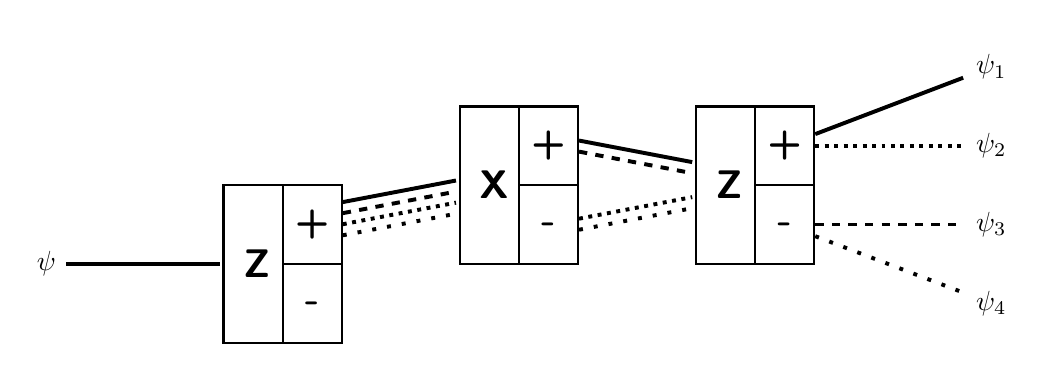
\begin{tikzpicture}[shorten >=1pt,auto, thick,
     square node/.style={rectangle, minimum height=2cm, minimum width=1.50cm, text width = 1cm, draw, font=\sffamily\Large\bfseries},
     port/.style={rectangle, draw,  minimum height=1cm, minimum width=0.75cm, font=\sffamily\Large\bfseries},
     wf/.style={rectangle, minimum height=1cm}]
    \apparatus{1}{3}{0}{Z};
    \apparatus{2}{6}{1}{X};
    \apparatus{3}{9}{1}{Z};

    \node[wf] (w0) at (0,0) {$\ket{\psi}$};
    \node[wf] (w1) at (12,2.5) {$\ket{\psi_1}$};
    \node[wf] (w2) at (12,1.5) {$\ket{\psi_2}$};
    \node[wf] (w3) at (12,0.5) {$\ket{\psi_3}$};
    \node[wf] (w4) at (12,-0.5) {$\ket{\psi_4}$};

    \draw[line width=0.5mm] (w0) -- (1);

    \draw[transform canvas={yshift=-0.6em}, line width=0.5mm, loosely dotted] (1+) -- (2);
    \draw[transform canvas={yshift=-0.2em}, line width=0.5mm, dotted] (1+) -- (2);
    \draw[transform canvas={yshift=0.2em}, line width=0.5mm, dashed] (1+) -- (2);
    \draw[transform canvas={yshift=0.6em}, line width=0.5mm] (1+) -- (2);

    \draw[transform canvas={yshift=-0.4em}, line width=0.5mm, loosely dotted] (2-) -- (3);
    \draw[transform canvas={yshift=0em}, line width=0.5mm, dotted] (2-) -- (3);
    \draw[transform canvas={yshift=0em}, line width=0.5mm, dashed] (2+) -- (3);
    \draw[transform canvas={yshift=0.4em}, line width=0.5mm] (2+) -- (3);

    \draw[line width=0.5mm, loosely dotted] (3-) -- (w4);
    \draw[line width=0.5mm, dashed] (3-) -- (w3);
    \draw[line width=0.5mm, dotted] (3+) -- (w2);
    \draw[line width=0.5mm] (3+) -- (w1);
\end{tikzpicture}
\caption[Insert an abbreviated caption here to show in the List of Figures]
{TODO: create section to discuss this example, and how it creates an inconsistent set of histories. Describe how the set can be made to be consistent}
\label{Figure:Intro:FigureExampleE}
\end{figure}
